\RequirePackage{luatex85}
\documentclass{standalone}

\usepackage{fontspec, unicode-math}
\setsansfont[Scale=MatchLowercase]{TeX Gyre Heros}
\setmathfont{TeX Gyre Termes Math}

\usepackage{pgfplots}
\pgfplotsset{compat=1.14}

\tikzset{
  every picture/.style={font={\sffamily\normalsize}, >=stealth},
  every pin edge/.style={black}}

\begin{document}

  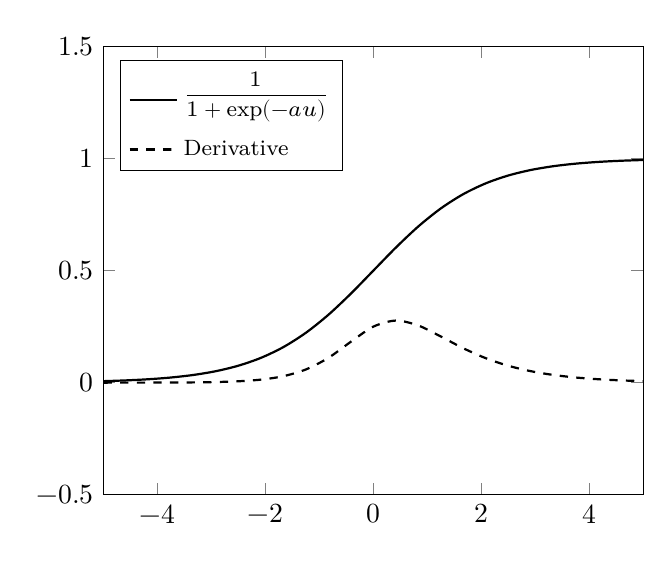
\begin{tikzpicture}
    \begin{axis}[%
        xmax = 5,
        xmin = -5,
        ymax = 1.5,
        ymin = -0.5,
        every axis plot/.style={thick, smooth},
        legend style={font=\footnotesize},
        legend pos=north west,
        legend cell align = left]

      \addplot[solid]  {1 / (1 + exp(-x))};
      \addplot[dashed] {(1 / (1 + exp(-x * 2))) * (1 - (1 / (1 + exp(-x))))};

      \legend{[text depth=1em]$\displaystyle \frac{1}{1 + \exp(-au)}$, Derivative}
    \end{axis}
  \end{tikzpicture}

\end{document}
